
From the viewpoint of scientific discovery, it comes quite so often that we would like to predict and study the behaviours of new materials, for which no parameterised energy function [\emph{c.f.} \cref{eq:total_energy_atom_pos_expand}] exists. Fortunately, quantum mechanics provides us with a fundamental theory which says, given a system with $m$ atoms containing $n$ electrons, its total energy can be, in principle, determined by the \emph{non-parameterised many-body} Schr\"{o}dinger equation that accounts for the interaction energies amongst all the nuclei and electrons in the material:
\begin{equation}\label{eq:full_Sch_eqn}
\left[\hat{\mathcal{K}}_N+\hat{\mathcal{K}}_e+\hat{\mathcal{V}}_{Ne}+\hat{\mathcal{V}}_{NN}+\hat{\mathcal{V}}_{ee}\right]\psi\left(\{\bm{R}\},\{\bm{r}\}\right)=E\psi\left(\{\bm{R}\},\{\bm{r}\}\right),
\end{equation}
the solution of which is the system \emph{wavefunction} $\psi\left(\{\bm{R}\},\{\bm{r}\}\right)$ that completely determines its quantum state with the given nuclei and electron coordinates, $\{\bm{R}\}$ and $\{\bm{r}\}$, respectively. The left-hand-side of \cref{eq:full_Sch_eqn} expresses the total system energy $E$ as sum of different energetic components, that are written in the form of \emph{operators}, including:
\begin{enumerate}
    \item The nuclear kinetic energy operator $\hat{\mathcal{K}}_N=\displaystyle{-\sum_{j=1}^{m}\frac{\hbar}{2M_j}\nabla_j^2}$, where $M_j$ is the nuclear mass for atom $j$, $\hbar$ is the Planck's constant and $m$ is the total number of atoms in the system.
    \item The electron kinetic energy operator $\hat{\mathcal{K}}_e=\displaystyle{-\sum_{i=1}^{n}\frac{\hbar}{2m_e}\nabla_i^2}$ with $m_e$ being the mass of electron and $n$ is the total number of electrons considered in the system.
    \item The  Coulomb attraction between nuclei and electrons $\hat{\mathcal{V}}_{Ne}=-\displaystyle{\sum_{i,j}\frac{e^2}{4\pi\epsilon_{0}}\frac{Z_j}{\left\vert \bm{r}_i-\bm{R}_{j}\right\vert}}$, here $\epsilon_{0}$ is the vacuum permittivity and $Z_j$ is the nuclear charge of the atom $j$.
    \item The Coulomb repulsion between nuclei  $\hat{\mathcal{V}}_{NN}=\displaystyle{\sum_{j<j^\prime}\frac{e^2}{4\pi\epsilon_{0}}\frac{Z_j Z_{j^\prime}}{\left\vert \bm{R}_{j^\prime}-\bm{R}_{j}\right\vert}}$, and
    \item The Coulomb repulsion between electrons $\hat{\mathcal{V}}_{ee}=\displaystyle{\sum_{i<i^\prime}\frac{e^2}{4\pi\epsilon_{0}}\frac{1}{\left\vert \bm{r}_{i^\prime}-\bm{r}_{i}\right\vert}}$.
\end{enumerate}



Since the nuclei are much heavier and move slower than the electrons, solving the Schr\"{o}dinger equation typically invokes the \emph{Born-Oppenheimer (BO) approximation} which drops the $\hat{\mathcal{K}}_N$ term, and treats $\hat{\mathcal{V}}_{NN}$ classically as a constant background electrostatic potential. However, exceptions do exist, such as the motion of light-weighted hydrogen atoms that plays a key role in hydrogen bonding, where the nuclei must also be treated quantum mechanically.\cite{ceriotti2016nuclear} which is beyond the focus of the present review. With this, \cref{eq:full_Sch_eqn} reduces to the following form for the electronic wavefunction $\psi(\left\{\bm{r}\right\})$ (note that the curly brackets are kept here to emphasise that this is a function of the collection of Cartesian coordinates for all the electrons in the system):
\begin{equation}\label{eq:e_Sch_eqn}
\left[\hat{\mathcal{K}}_e+\hat{\mathcal{V}}_{Ne}+\hat{\mathcal{V}}_{ee}\right]\psi\left(\{\bm{r}\}\right)=E\psi\left(\{\bm{r}\}\right).
\end{equation}

\begin{figure}[htb]    
    \centering
    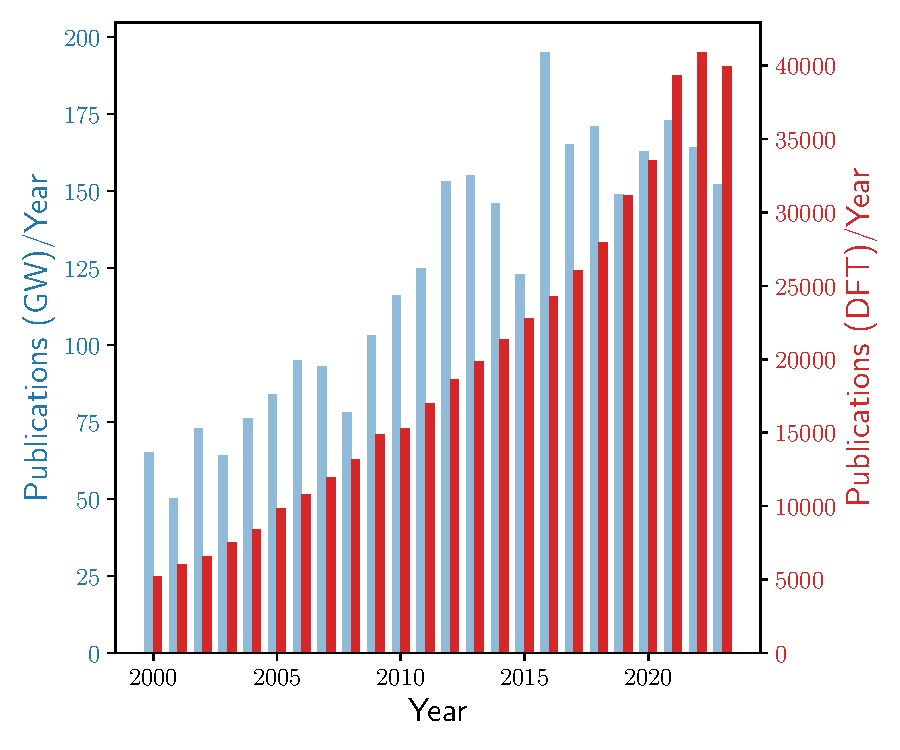
\includegraphics[width=0.48\textwidth]{DFT_statistics.pdf}
    \caption{Number of publications per year since 2000 which involve `Density Functional' or `DFT' according to the Web of Science. In comparison, the same trend for publications including `GW approximations' is also shown.}
    \label{fig:DFT_statistics}
\end{figure}
However, even with the BO-approximation, \cref{eq:e_Sch_eqn} is still intractable to be solved for realistic materials, for instance, it is estimated that $\sim10^{46}$ complex numbers are necessary to fully specify the wavefunction  of the 10 valence electrons for crystalline silicon containing two atoms in its cubic unit cell with a cell length of 5.42 $\mbox{\AA}$.\cite{giustino2014materials} Fortunately, the formulation and development of the  Density Functional Theory (DFT) have provided a practical solution to overcome such a challenge and has become the backbone of modern material theory and discoveries [\cref{fig:DFT_statistics}]. Note that, although  Density Functional \emph{Theory} is the most commonly used term in the literature, what it really encompasses, are the formally exact Hohenberg-Kohn-Sham (HKS) theorems, and the Density Functional \textit{Approximations} (DFAs) that brings the theory into practicalities, and these will be followed and briefly reviewed in the following two sections.